% LaTeX document on "The Pandemic and Software Development" with TikZ/PGF
\documentclass{article}
\usepackage{tikz}
\usepackage{pgfplots}
\usepackage{pgfplotstable}
\pgfplotsset{compat=1.18}

\title{The Pandemic and Software Development}
\author{Sebasg.code}
\date{\today}

\begin{document}

\maketitle

\section{Introduction}
The COVID-19 pandemic had a profound impact on multiple industries, including software development. This document explores how the pandemic highlighted the shortage of developers, influenced salaries and job availability, brought changes to the software development field, and increased interest in studying software-related disciplines.

\section{Developer Shortages During the Pandemic}
The pandemic exposed a significant gap in the demand and availability of skilled software developers. As companies accelerated their digital transformations, the demand for developers surged, leaving many positions unfilled.

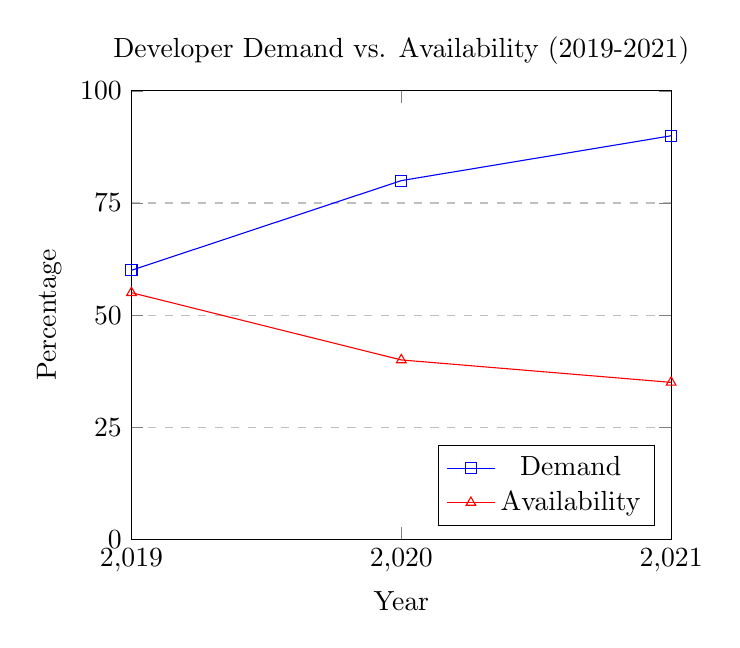
\begin{tikzpicture}
\begin{axis}[
    title={Developer Demand vs. Availability (2019-2021)},
    xlabel={Year},
    ylabel={Percentage},
    xmin=2019, xmax=2021,
    ymin=0, ymax=100,
    xtick={2019, 2020, 2021},
    ytick={0, 25, 50, 75, 100},
    legend pos=south east,
    ymajorgrids=true,
    grid style=dashed,
]
\addplot[
    color=blue,
    mark=square,
]
coordinates {
    (2019, 60)
    (2020, 80)
    (2021, 90)
};
\addplot[
    color=red,
    mark=triangle,
]
coordinates {
    (2019, 55)
    (2020, 40)
    (2021, 35)
};
\legend{Demand, Availability}
\end{axis}
\end{tikzpicture}

\section{Impact on Salaries and Job Availability}
As demand outpaced supply, salaries for software developers increased significantly, while the competition for talent became fierce.

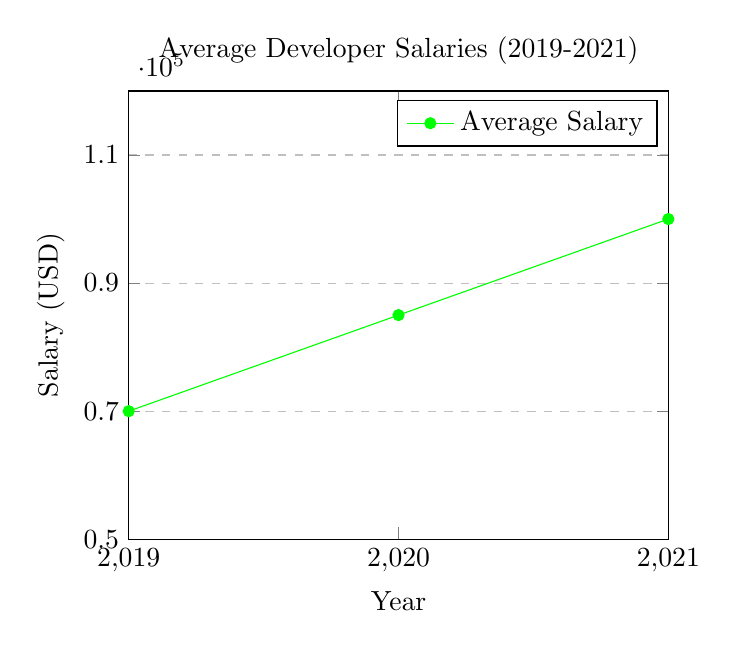
\begin{tikzpicture}
\begin{axis}[
    title={Average Developer Salaries (2019-2021)},
    xlabel={Year},
    ylabel={Salary (USD)},
    xmin=2019, xmax=2021,
    ymin=50000, ymax=120000,
    xtick={2019, 2020, 2021},
    ytick={50000, 70000, 90000, 110000},
    ymajorgrids=true,
    grid style=dashed,
]
\addplot[
    color=green,
    mark=* ,
]
coordinates {
    (2019, 70000)
    (2020, 85000)
    (2021, 100000)
};
\legend{Average Salary}
\end{axis}
\end{tikzpicture}

\section{Post-Pandemic Changes for Developers}
The pandemic brought long-lasting changes to the software development landscape, including:
\begin{itemize}
    \item Remote work becoming the norm.
    \item Increased focus on cybersecurity.
    \item Emphasis on collaboration tools and DevOps practices.
\end{itemize}

\section{Growth in Software-Related Education}
The demand for developers inspired many individuals to pursue studies in software-related fields. The following graph illustrates the enrollment growth in software development programs globally:

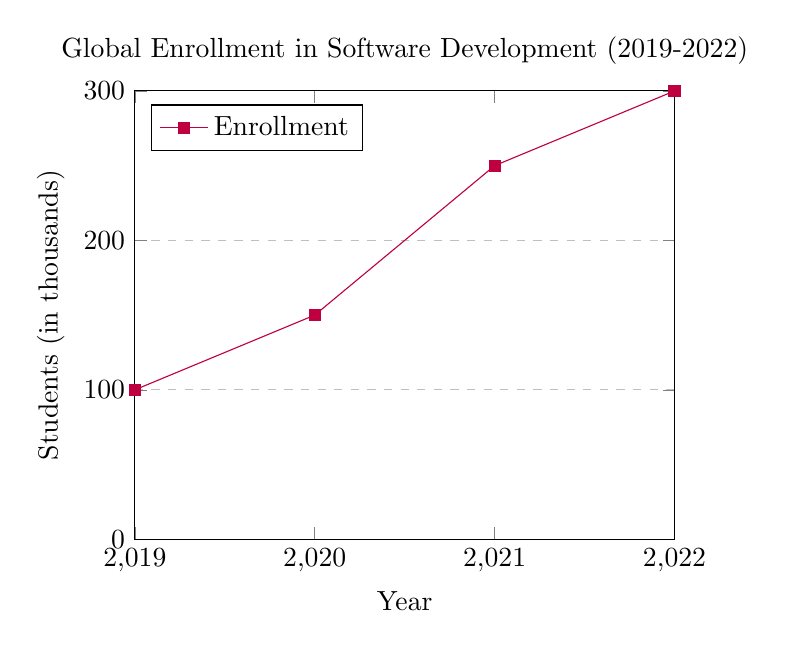
\begin{tikzpicture}
\begin{axis}[
    title={Global Enrollment in Software Development (2019-2022)},
    xlabel={Year},
    ylabel={Students (in thousands)},
    xmin=2019, xmax=2022,
    ymin=0, ymax=300,
    xtick={2019, 2020, 2021, 2022},
    ytick={0, 100, 200, 300},
    legend pos=north west,
    ymajorgrids=true,
    grid style=dashed,
]
\addplot[
    color=purple,
    mark=square*,
]
coordinates {
    (2019, 100)
    (2020, 150)
    (2021, 250)
    (2022, 300)
};
\legend{Enrollment}
\end{axis}
\end{tikzpicture}

\section{Regional and Sector-Specific Analysis}
The impact of the pandemic on software development varied across regions and sectors. The table below shows the demand growth in different regions:

\begin{tikzpicture}
\pgfplotstabletypeset[
    col sep=comma,
    string type,
    every head row/.style={
        before row=\hline,after row=\hline},
    every last row/.style={after row=\hline},
]{
Region,2019,2020,2021
North America,70,85,90
Europe,60,75,80
Asia,50,70,75
South America,40,60,65
Africa,30,50,55
}
\end{tikzpicture}

\section{Future Predictions}
Looking ahead, the software development industry is expected to:
\begin{itemize}
    \item See continued salary growth due to persistent demand.
    \item Experience a 15\% annual increase in developer roles globally.
    \item Witness more students enrolling in specialized fields like AI, data science, and cybersecurity.
\end{itemize}

The graph below projects the global growth in software-related fields:

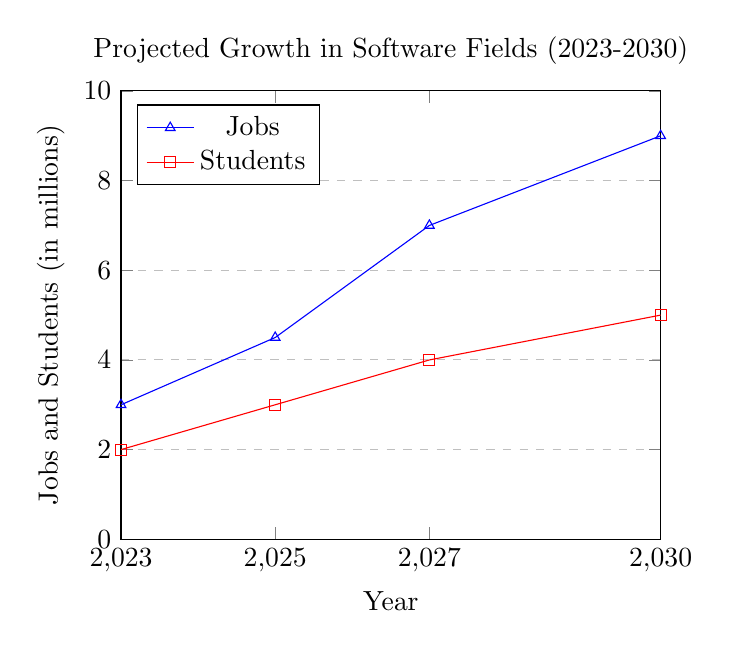
\begin{tikzpicture}
\begin{axis}[
    title={Projected Growth in Software Fields (2023-2030)},
    xlabel={Year},
    ylabel={Jobs and Students (in millions)},
    xmin=2023, xmax=2030,
    ymin=0, ymax=10,
    xtick={2023, 2025, 2027, 2030},
    ytick={0, 2, 4, 6, 8, 10},
    legend pos=north west,
    ymajorgrids=true,
    grid style=dashed,
]
\addplot[
    color=blue,
    mark=triangle,
]
coordinates {
    (2023, 3)
    (2025, 4.5)
    (2027, 7)
    (2030, 9)
};
\addplot[
    color=red,
    mark=square,
]
coordinates {
    (2023, 2)
    (2025, 3)
    (2027, 4)
    (2030, 5)
};
\legend{Jobs, Students}
\end{axis}
\end{tikzpicture}

\section{Conclusion}
The COVID-19 pandemic underscored the importance of software development in a rapidly digitalizing world. By highlighting developer shortages, driving salary increases, and inspiring educational interest, it has fundamentally reshaped the industry. Continued adaptation and innovation will define the future of software development as the world embraces further digital transformation.

\end{document}
